\subsection{Real Estate Investments}

\subsubsection{Overview of Real Estate Investments}

\begin{remark} \hlt{Types of Real Estate}
\begin{enumerate}[label=\roman*.]
\setlength{\itemsep}{0pt}
\item Residential: single-family homes, apartments, condominiums, manufactured housing
\item Non-Residential Property: office, shopping centres, factories, warehouses, agriculture, specialty real estate
\end{enumerate}
\end{remark}

\begin{figure}[H]
\centering
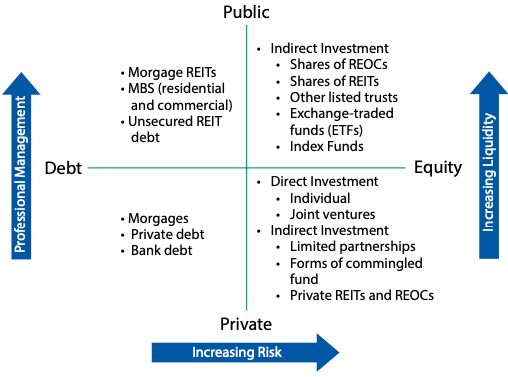
\includegraphics[scale=0.4]{/alts/reinvestments}
\caption{Forms of Real Estate Investments}
\end{figure}

\begin{remark} \hlt{Private vs Public Real Estate}
\begin{enumerate}[label=\roman*.]
\setlength{\itemsep}{0pt}
\item Public Real Estate: ownership on securities that serve as claims on underlying.
\begin{enumerate}[label=\arabic*.]
\setlength{\itemsep}{0pt}
\item Real Estate Investment Trust (REIT): restricted to primarily owning and operating rental properties, or purchasing mortgages. Required to distribute all earnings to avoid paying corporate income taxes.
\item Real Estate Operating Company (REOC): taxable corporations that operate and manage commercial real estate with few corporate-structure restrictions. Own and often develop real estate.
\item Mortgage-Backed Securities (MBS): classified as public investments when there are active secondary trading markets. Restrictions exist as to purchase eligibility and minimum trade sizes. Trust certificate owners (bondholders) typically own right to receive cash flow from underlying pool of mortgages, which are secured by real property.
\end{enumerate}
\item Private Real Estate: direct investment by purchasing property or lending money to purchaser. Can be solely owned or owned through partnerships, where GP provides property management services.
\end{enumerate}
\end{remark}

\begin{remark} \hlt{Capital Position}
\begin{enumerate}[label=\roman*.]
\setlength{\itemsep}{0pt}
\item Equity investor has ownership interest in real estate or securities of an entity that owns real estate. Controls decisions such as borrowing money, property management, exit strategy.
\item Debt investor owns mortgage or mortgage securities, usually secured by the underlying. Lender has superior claim over equity investor during default.
\end{enumerate}
As lender has to be repaid first, value of equity interest is value of property less outstanding debt.
\end{remark}

\begin{remark} \hlt{Characteristics of Real Estate Investment}
\begin{enumerate}[label=\roman*.]
\setlength{\itemsep}{0pt}
\item Heterogeneity: no two RE are the same due to size, age, construction materials, tenants, lease terms
\item High Unit Value: RE is indivisible, unit value is higher, hence difficult to construct diversified portfolio
\item Active Management: private Re investment require active property management, which involves maintenance, negotiating leases, collection of rents
\item High Transaction Costs: involves appraisers, lawyers, brokers, construction personnel
\item Depreciation: less desirable due to location, design, or obsolescence. Deductibility of depreciation for tax purposes is attractive feature for investors in most jurisdictions
\item Illiquidity: takes time to market and complete sale of property
\item Need for Debt Capital: due to high costs of acquisition. RE values are lower when interest rates are high and debt capital is scarce
\item Price Determination: due to heterogeneity and low transaction volume, appraisals are required, which is based on similar but not identical properties. Market is less efficient. Limited participants, importance  of local knowledge, makes it harder to know market value of a property
\end{enumerate}
\end{remark}

\begin{remark} \hlt{Demand and Supply Risk Factors of Commercial Real Estate}
\begin{enumerate}[label=\roman*.]
\setlength{\itemsep}{0pt}
\item Business Conditions: GDP, employment, household income, interest rates, inflation affect rental
\item Demographics: shifts in size and age distribution affect type of property in demand. Changes in socioeconomic groups and rate of new household formation all affect demand.
\item Excess Supply: market conditions can change significantly while approvals are obtained, while property is completed, and when property is fully leased.\\
During lead time, if market conditions weaken, lower demand affects rents and vacant rates, resulting in lower returns. Commercial property demand coincide with business cycle.
\end{enumerate}
\end{remark}

\begin{remark} \hlt{Valuation Risk Factors of Commercial Real Estate}
\begin{enumerate}[label=\roman*.]
\setlength{\itemsep}{0pt}
\item Cost and Availability of Capital: RE must compete with other investments for capital. Demand for RE is reduced when debt capital is scarce, interest rates are high.
\item Availability of Information: lack of info to conduct property analysis adds to risk of investment. Availability of data depends on country. More information is available as RE investments become more global.
\item Lack of Liquidity: due to size and complexity of transactions, due diligence takes time and is costly. Quick sale will require significant discount.
\item Interest Rates: RE values may initially decline when interest rates rise, but may increase over time through the latter part of the RE cycle.
\end{enumerate}
\end{remark}

\begin{remark} \hlt{Operational Risk Factors of Commercial Real Estate}
\begin{enumerate}[label=\roman*.]
\setlength{\itemsep}{0pt}
\item Management Expertise: property managers and asset managers must take important operational decisions, such as lease negotiation, property maintenance, marketing, property renovation.
\item Lease Provisions: pre-determined contractual rent step-ups can move in line with unexpected inflation if tied to consumer price or other inflation-linked index. Expense caps will limit how much of annual increase of operating expenses is passed to tenant. Short-term leases allow periodic rent reviews in response to changing market conditions.
\item Leverage: use of leverage to finance real estate affect returns but not value of underlying RE. Loan-to-value (LTV) ratio (ratio of borrowed funds to total purchase price) measure leverage, with higher LTV resulting in higher leverage hence higher risk. With leverage, small decrease in net operating income (NOI) negatively magnifies amount of CF available to equity investors after debt service.
\item ESG Considerations: RE values may be affected by environmental conditions. Social and governance-related issues may impact development and management of RE.
\item Obsolescence: Changes in tenant preferences, regulations, technology affect space demand. May not be economically viable to upgrade, reconfigure, or repurpose old buildings to comply with energy efficiency and other modernisation requirements or changing business and consumer preferences.
\item Market Disruptions: new innovations such as remote working, online shopping, same-day delivery and other disruptions affect the demand for various kinds of real estate.
\item Other Risk Factors: unobserved physical defects in property, natural disasters, pandemics, terrorism, climate change may be unidentified and difficult-to-forecast at time of purchase.
\end{enumerate}
\end{remark}

\begin{remark} \hlt{Reasons to Invest in Real Estate}
\begin{enumerate}[label=\roman*.]
\setlength{\itemsep}{0pt}
\item Current Income: earn income from letting, leasing, or renting, after paying operating expenses, financing costs, and taxes. Usually largest component of investor return.
\item Capital Appreciation: property values may increase over time, which forms part of total return
\item Inflation Hedge: both rents and property values expected to rise in inflationary environment
\item Diversification: not typically highly correlated with performance of other asset classes, hence may reduce risk relative to expected return. Publicly traded RE behaves more like stock in the short-run.
\item Tax Benefits: private RE investments may receive favourable tax treatment. In US, RE can be depreciated for tax purposes faster than actual life. In some countries, REITs do not may income taxes if income is distributed ($> 90\%$) to shareholders.
\end{enumerate}
\end{remark}

\begin{remark} \hlt{Role of Real Estate in Portfolio}\\
RE has both bond and stock characteristics. Leases call for periodic rental payments, similar to coupon payments of a bond. As lease expires, there is uncertainty on renewal and future rental rates. Availability of competing space, tenant profitability, state of overall economy affect this uncertainty just as these factors affect stock prices. Hence RE risk-return profile is between risk-return profile of stocks and bonds.
\end{remark}

\begin{remark} \hlt{Core Investing Style}\\
A conservative strategy that limits investments to high quality and low leverage ($< 30\%$ LTV), and avoids speculative risks in favour of steady returns.
\end{remark}

\begin{remark} \hlt{Economic Value Determinants of Real Estate Investments}\\
National GDP growth is largest driver of economic value for all RE types, as this means more jobs, greater need for office space, more disposal income, more growth in shopping centres, greater demand for hotel rooms etc.
\end{remark}

\begin{flushleft}
Economic Value Determinants
\begin{tabularx}{\textwidth}{p{10em}|p{12em}|p{6em}|p{2.5em}|p{2.5em}|p{2.5em}|p{4.5em}}
\hline
\rowcolor{gray!30}
Factor Type & Factor & Multi-Family & Retail & Hotel & Office & Industrial \\
\hline
Macro & GDP Growth & $\checkmark$ & $\checkmark$ & $\checkmark$ & $\checkmark$ & $\checkmark$ \\
& Population Growth & $\checkmark$ & $\checkmark$ & $\checkmark$ & $\checkmark$ & $\checkmark$ \\
& Job Creation & $\checkmark$ & $\checkmark$ & $\checkmark$ & $\checkmark$ & $\checkmark$ \\
& Wage Growth & $\checkmark$ & $\checkmark$ & $\checkmark$ & $\checkmark$ & $\checkmark$ \\
& Regulatory & $\checkmark$ & $\checkmark$ & $\checkmark$ & $\checkmark$ & $\checkmark$ \\
& Taxes & $\checkmark$ & $\checkmark$ & $\checkmark$ & $\checkmark$ & $\checkmark$ \\
\hline
Individual & Household Formations & $\checkmark$ & $\checkmark$ & & & \\
& Personal Income & $\checkmark$ & $\checkmark$ & $\checkmark$ & & \\
& Consumer Confidence & $\checkmark$ & $\checkmark$ & $\checkmark$ & & \\
& Consumer Credit & $\checkmark$ & $\checkmark$ & $\checkmark$ & & \\
\hline
Business Environment & Retail Sales Growth & & $\checkmark$ & & & $\checkmark$ \\
& Consumer Spending & & $\checkmark$ & $\checkmark$ & & $\checkmark$ \\
& Business Formations & $\checkmark$ & & $\checkmark$ & $\checkmark$ & $\checkmark$ \\
& Business Investment & & & $\checkmark$ & $\checkmark$ & $\checkmark$ \\
& Business Confidence & & $\checkmark$ & $\checkmark$ & $\checkmark$ \\
\hline
Industrial & Industrial Production & & & & & $\checkmark$ \\
& Trade, Transport, Logistics & & & & & $\checkmark$ \\
& Changing Supply Routes & & & & & $\checkmark$ \\
\hline
\end{tabularx}
\end{flushleft}

\begin{remark} \hlt{Types of Leases}
\begin{enumerate}[label=\roman*.]
\setlength{\itemsep}{0pt}
\item Net Lease: tenant responsible for paying operating expenses.
\item Gross Lease: owner to pay operating expenses.
\item Triple-Net Lease (NNN): tenants to pay for share of common area maintenance (CAM) and repair expenses, property taxes, building insurance costs; also responsible for own furnishings, equipment, systems etc. against fire, water damage, and other perils.
\item Sales-Leaseback: long-term single-tenant lease requiring tenant to pay all expenses directly, in addition to base rent. Company sells building it owns and occupies to a RE investor and the company then signs long-term least with buyer to continue to occupy the building.
\end{enumerate}
\end{remark}

\begin{remark} \hlt{Commercial Property Classifications}
\begin{enumerate}[label=\roman*.]
\setlength{\itemsep}{0pt}
\item Residual Properties: multi-family and single-family properties that are not owner occupied, purchased with the intent to rent out to produce income.\\
Multi-family properties differentiated by location (urban, suburban), structure height (high-rise, mid-rise, low-rise, garden apartments, townhouses), amenities (pool, balcony, exercise facilities, concierge services).\\
Demand depends on population growth. Age demographic vary by country, type of property, locale. Cost of buying versus cost of renting, measured by ratio of home prices to rents, also affect demand.
\item Office: multi-tenant, or single-tenant. Built with needs of specific tenants in mind.\\
Demand heavily dependent on job growth, especially in industries that are heavy users of office space. Average length of office leases varies globally.
\item Industrial and Warehouse: wholesale and retail distribution centres, combination warehouse/showroom and office buildings, light or heavy manufacturing facilities and associated warehouse space.\\
Demand heavily dependent on overall economy. Import and export activities also affect demand.\\
Net leases are common.
\item Retail: vary significantly in size. Large regional shopping centres, malls with large department stores, big-box retailers, neighbourhood shopping centres, standalone properties.\\
Demand heavily dependent on consumer spending, which in turn depends on overall economy, job growth, population growth, savings rates.\\
Retail lease terms vary by quality of property, size and importance of tenant.\\
Retail tenant often required to pay additional rent when sales reach certain level (percentage lease or rent). Lease will specify minimum amount of rent to be paid without regard to sales. 
\item Hospitality: varies by size and available amenities. Motels, smaller hotels, resort hotels etc.
\item Other Specialty Types: hospitals, bioscience laboratories, self-storage, student housing, cell towers, data centres, parking facilities, marinas, sport complexes etc.
\end{enumerate}
Low-risk commercial property types include office, industrial/warehouse, retail, multi-family. Hospitality properties are riskier as leases are not used, and performance is highly correlated with business cycle.
\end{remark}

\begin{remark} \hlt{Property Due Diligence: Market Review}
\begin{enumerate}[label=\roman*.]
\setlength{\itemsep}{0pt}
\item Understand market trends, including local market population, job and income growth
\item Understand expected additions to supply and space absorption rates (how much net space is leased yearly)
\item Understand tenant preferences, building amenities, market rents, and expense trends.
\end{enumerate}
\end{remark}

\begin{remark} \hlt{Property Due Diligence: Lease and Rent Review}
\begin{enumerate}[label=\roman*.]
\setlength{\itemsep}{0pt}
\item Compare the tenant rents with market rent forecasts and lease length to determine how much rents will change when leases expire.
\item Review lease expiration timeline for all tenants. $~20\%$ of leases expire in any given year, or there may be some years with larger lease expirations.
\item Analyse the history of rental payments, late payments, and any defaults for the major tenants.
\end{enumerate}
\end{remark}

\begin{remark} \hlt{Property Due Diligence: Review Costs of Re-Leasing}\\
Review costs and incentives provided to both renewing and new tenants.
\begin{enumerate}[label=\roman*.]
\setlength{\itemsep}{0pt}
\item Costs: typically include commissions paid to real estate brokers and downtime between leases.
\item Incentives: typically include a period of free rent and allowances for tenant improvements to their space.
\end{enumerate}
These costs are typically not included in annual operating income. Instead, these expenses are capitalised and amortised over the length of the lease.
\end{remark}

\begin{remark} \hlt{Property Due Diligence: Review Documentation}
\begin{enumerate}[label=\roman*.]
\setlength{\itemsep}{0pt}
\item Review copies of bills for operating expenses, i.e., utility bills and real estate taxes.
\item Review multiple years of audited fin statements. CFS provide details on Opex and revenue trends.
\item Look for evidence of overstated income (Capex underspending) or occupancy (tenant incentives).
\end{enumerate}
\end{remark}

\begin{remark} \hlt{Property Due Diligence: Property Inspections and Service Agreements}
\begin{enumerate}[label=\roman*.]
\setlength{\itemsep}{0pt}
\item Conduct environmental inspection to check for issues, i.e., contaminant material.
\item Conduct physical and engineering inspection for structural issues. Check condition of systems, structures, and foundation and  adequacy of utilities.
\item Review service and maintenance agreements to determine whether recurring problems exist.
\item Conduct property survey to determine if the planned physical improvements are in the boundary lines of the site and to find out if any easements would affect the value.
\end{enumerate}
\end{remark}

\begin{remark} \hlt{Property Due Diligence: Legal Documentation and Tax Compliance}
\begin{enumerate}[label=\roman*.]
\setlength{\itemsep}{0pt}
\item Conduct title search by reviewing the ownership history. Make sure there are no issues related to the property title and that the property is not subject to any previously unidentified liens.
\item Verify that the property is compliant with zoning laws, environmental regulations, parking ratios etc.
\item Verify that property taxes, insurance, special assessments etc. have been paid.
\end{enumerate}
\end{remark}

\begin{method} \hlt{Appraisal-Based Indexes}\\
Index combine valuation from individual properties to provide measure of market movements.\\
In US, members of NCREIF (National Council of Real Estate Investment Fiduciaries) contribute appraised values, net operating income (NOI), capital expenditures and other information on a quarterly basis. The return for all properties is then calculated as
\begin{equation}
\text{Return} = \frac{\text{NOI} - Capex + (\text{Market Value}_{\text{End}} - \text{Market Value}_{\text{Beginning}})}{\text{Market Value}_{\text{Beginning}}} \nonumber
\end{equation}
The return is a holding-period return. The index is then value weighted based on returns of separate properties.
\end{method}

\begin{remark} \hlt{Characteristics of Appraisal-Based Indexes}\\
The index has a current yield component (NOI divided by beginning market value).\\
Remaining components of equation produce the capital return.\\
Note that the income component of return does not represent REIT distributions, unlike other asset classes.\\
The index lags actual transactions as transactions occur before appraisals are performed. The lag can be adjusted by un-smoothing the index or by using a transaction-based index.\\
Global RE index is a cap-weighted index that is published quarterly, and includes local currency return. Index combines data from US, Europe, and Asia.
\end{remark}

\begin{method} \hlt{Transaction-Based Indices}
\begin{enumerate}[label=\roman*.]
\setlength{\itemsep}{0pt}
\item Repeat-Sales Index: relies on repeat sales of same property. Change in market conditions can be measured once a property is sold more than once.\\
Regression may then be used to allocate change in value to each quarter.
\item Hedonic Index: requires only single sale data. Regression model controls for differences in property characteristics such as size, age, quality of construction, and location. Require a lot of data, most reliable at national level; may be reliable at regional level if sufficient transactions are available.
\end{enumerate}
\end{method}

\subsubsection{Publicly Traded Securities}